\section{Introduction}

\begin{frame}
\frametitle{Motivación}
\framesubtitle{El lenguaje de programación C}

\pause

Lenguaje C:

\pause

\begin{itemize}
\item{Cercanía  a la máquina y bajo \textit{overhead} permiten eficiencia.}
\pause
\item{Utilizado para sistemas operativos, aplicaciones de sistemas embebidos, compiladores, librerías e interpretadores.}
\pause
\end{itemize}

Desventaja?
\pause
\begin{itemize}
\item{Parte de la semántica se define en lenguaje natural, lo cual la hace vulnerable a ambigüedades.}
\end{itemize}

\end{frame}


\begin{frame}
\frametitle{Motivación}
\framesubtitle{Objetivos del trabajo}

\pause
\begin{itemize}
\item{Formalizar la semántica de un lenguaje imperativo que represente un subconjunto determinístico de la semántica de C.}
\pause
\item{Escribir un interpretador dentro del ambiente de Isabelle/HOL y demostrar su correctitud.}
\pause
\item{Generar código C a partir de programas escritos en la semántica formal.}
\pause
\item{Crear un ambiente de pruebas y una batería de pruebas que incrementen la confianza en el proceso de generación de código.}
\end{itemize}

\end{frame}


\begin{frame}
\frametitle{Chloe}
\framesubtitle{Un lenguaje imperativo, subconjunto de C}

\begin{columns}[t]
\column{.45\textwidth}
\begin{block}{Características:}
\pause
\begin{itemize}
\item{Variables}
\pause
\item{Arreglos}
\pause
\item{Aritmética de apuntadores}
\pause
\item{Ciclos}
\pause
\item{Condicionales}
\pause
\item{Funciones}
\pause
\item{Memoria dinámica}
\pause
\end{itemize}
\end{block}
\column{.45\textwidth}
\begin{block}{Limitaciones:}
\begin{itemize}
\pause
\item{Sistema de tipos estático correcto y completo}
\pause
\item{Concurrencia}
\pause
\item{Operaciones I/O}
\pause
\item{Goto}
\pause
\item{Etiquetas}
\pause
\item{Instrucciones break y continue}
\end{itemize}
\pause
\end{block}
\end{columns}

\end{frame}


\begin{frame}
\frametitle{Semántica}

\pause

Existen tres enfoques principales:

\pause

\begin{itemize}
\item{Operacional}
\pause
  \begin{itemize}
    \item{Pasos largos}
    \item{Pasos cortos}
  \end{itemize}
\pause
\item{Denotacional}
\pause
\item{Axiomática}
\pause
\end{itemize}

\end{frame}

\begin{frame}
\frametitle{Isabelle/HOL}

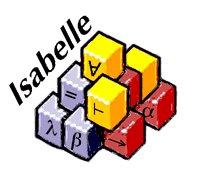
\includegraphics[scale=0.5]{images/isabelle.png}

\begin{itemize}
\item{Isabelle/HOL es un demostrador interactivo de teoremas escrito en ML.}
\pause
\item{Desarrollado por Larry Paulson y Tobias Nipkow.}
\pause
\item{Utiliza el lenguaje HOL para realizar las pruebas.}
\pause
\item{Permite hacer definiciones y demostrar propiedades acerca de las mismas.}
\pause
\item{Se usa la máquina para asistir en las demostraciones}
\pause
\end{itemize}

\end{frame}
